%\documentclass{beamer}
\documentclass[aspectratio=169]{beamer}
\usetheme{Boadilla}

%\usetheme{Warsaw}
%\setbeamercovered{transparent}
\beamertemplatetransparentcoveredhigh
\usepackage[portuges]{babel}
\usepackage[latin1]{inputenc}
\usepackage{lmodern}
\usepackage[T1]{fontenc}
\usepackage{hyperref} 
\usepackage[portuguese, linesnumbered, vlined, titlenumbered, ruled]{algorithm2e}

\newcommand{\eng}[1]{\textsl{#1}}
\newcommand{\cod}[1]{\texttt{#1}}

\title[Apresenta��o]{Curso Intelig�ncia Artificial: do Zero ao Infinito}
\author[Frederico Oliveira]{Transfer Learning}
\institute[UFMT]{Universidade Federal de Mato Grosso}
\date{}
%\titlegraphic{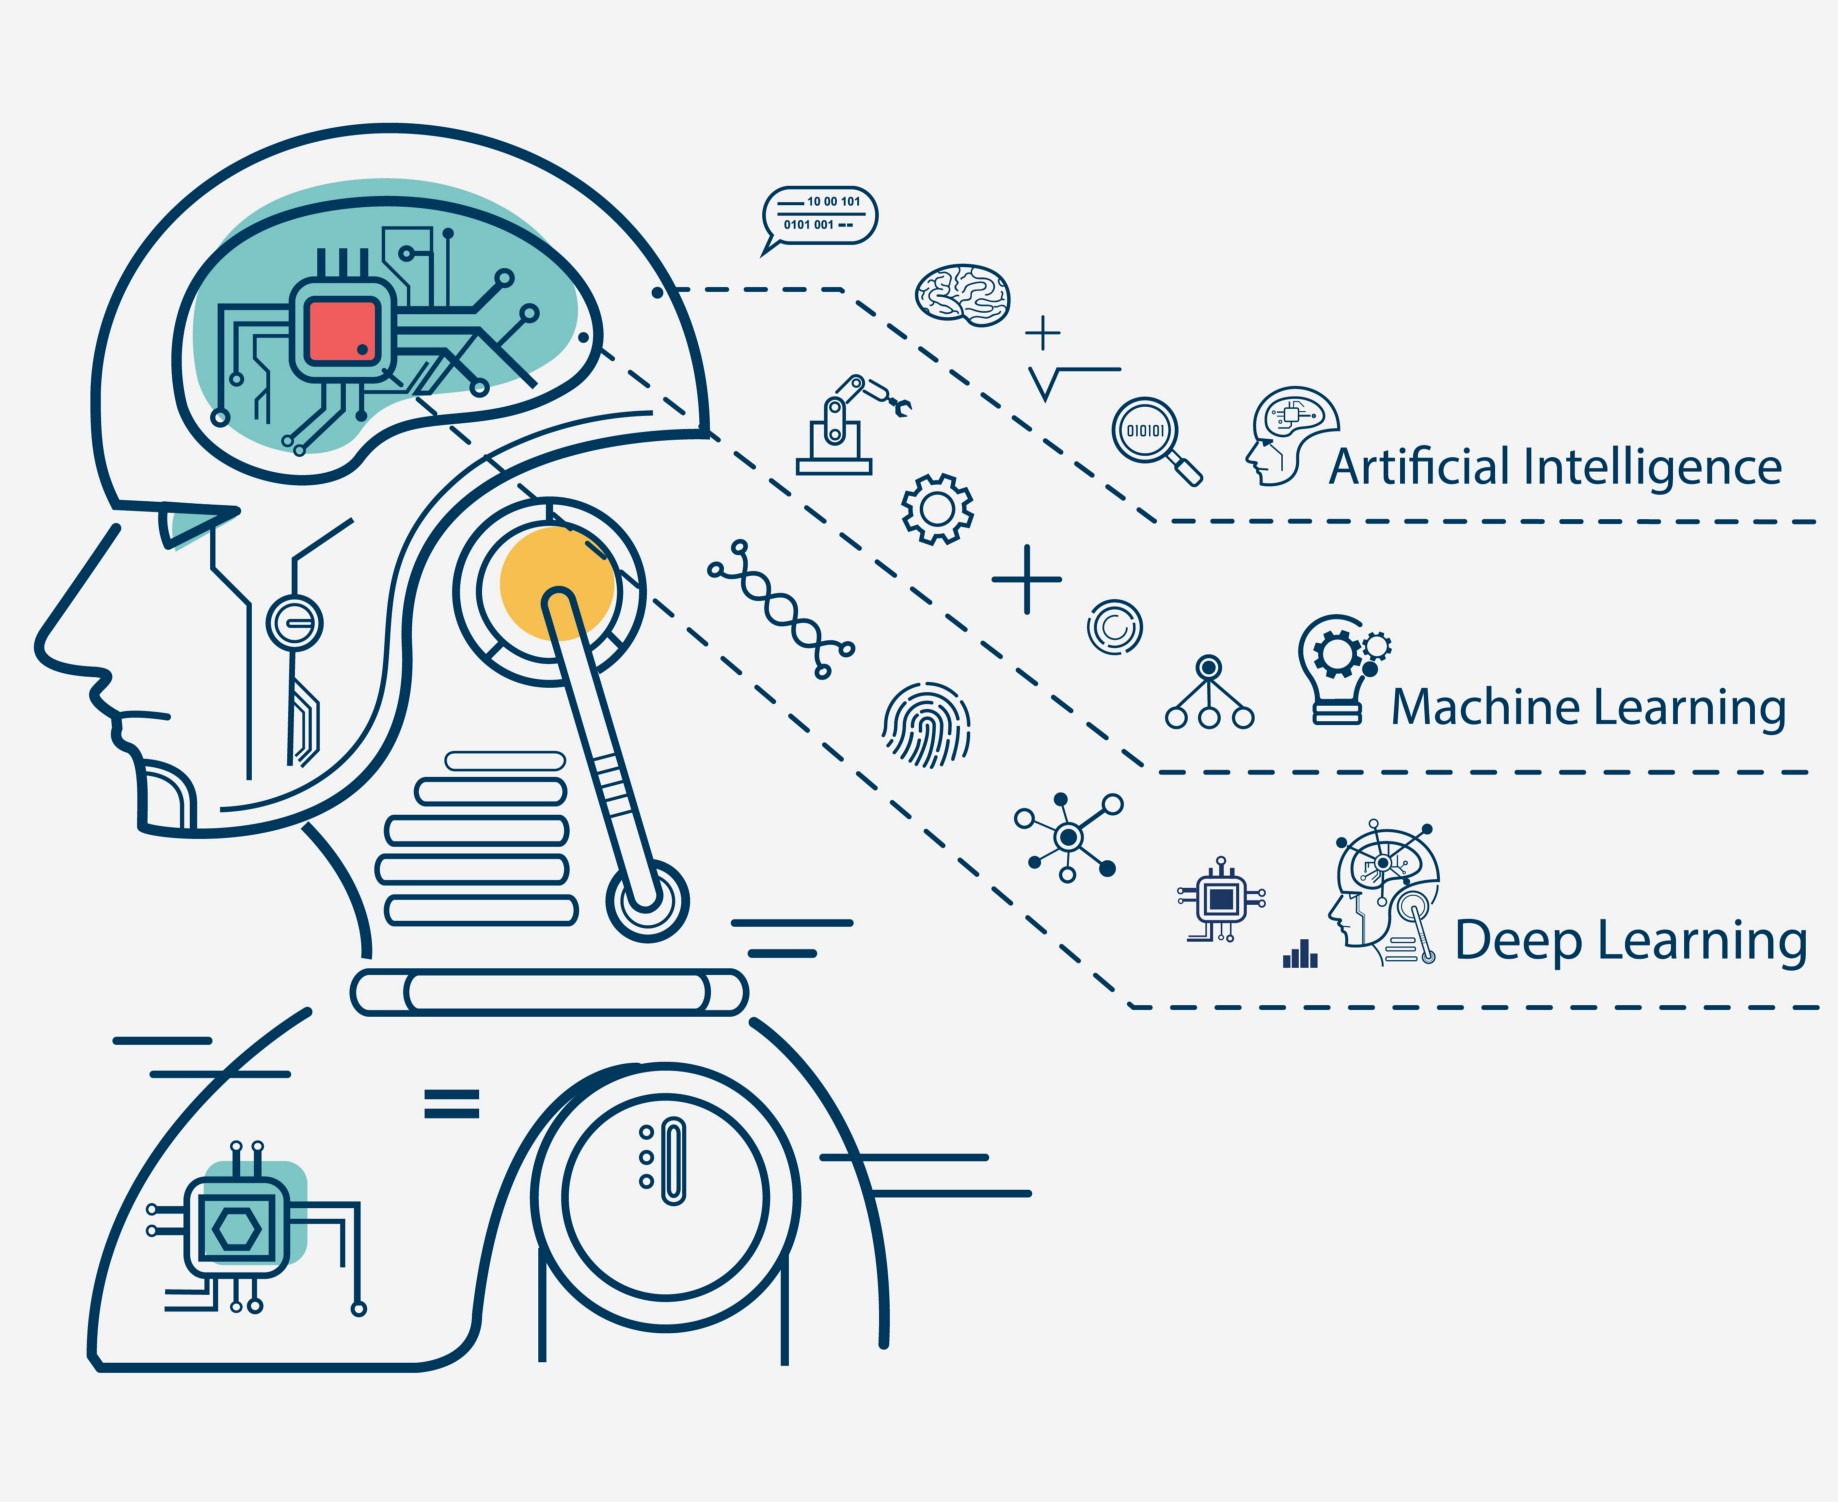
\includegraphics[width=\textwidth,height=.5\textheight]{imgs/intro.jpeg}}
%\usebackgroundtemplate{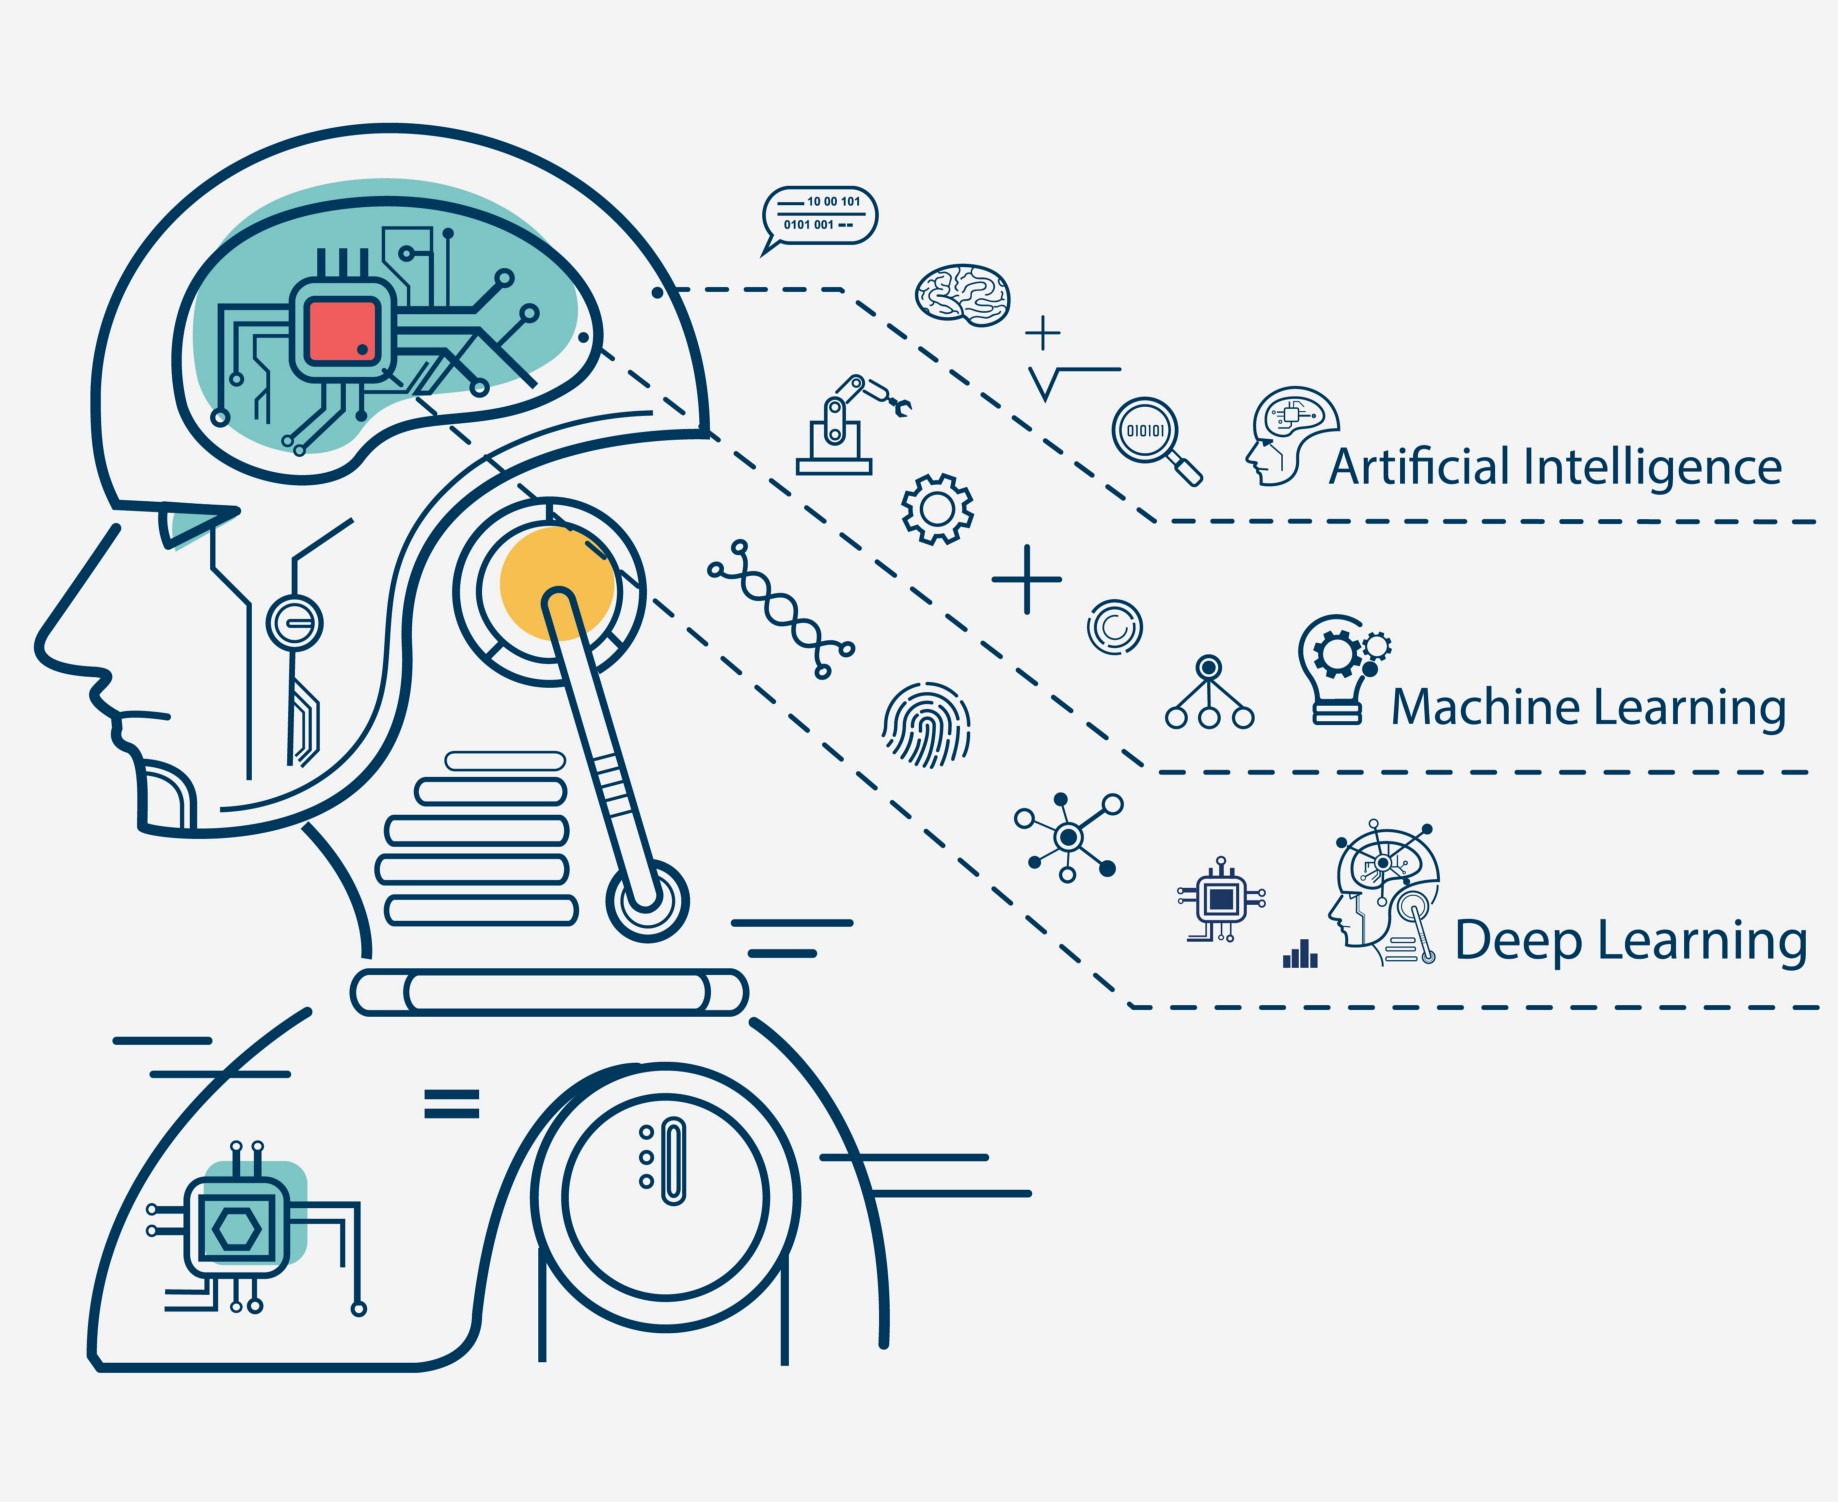
\includegraphics[width=\paperwidth]{imgs/intro.jpeg}}
\begin{document}

\begin{frame}[plain]
  \titlepage
\end{frame}

%
%\AtBeginSection[]
%{
%	\begin{frame}
%	\frametitle{Agenda}
%	\tableofcontents[currentsection]
%\end{frame}
%}


%%%%%%%%%%%%%%%%%%%%%%%%%%%%%%%%%%%%%%%%%%%%%%%%%%%%%%%%%%%%%%%%%%%%%%%%%%%%%%%%%%%%%%%%%%%%%%%%%%%%%%%%%%%%%%%%
%\section*{Roteiro}
%%%%%%%%%%%%%%%%%%%%%%%%%%%%%%%%%%%%%%%%%%%%%%%%%%%%%%%%%%%%%%%%%%%%%%%%%%%%%%%%%%%%%%%%%%%%%%%%%%%%%%%%%%%%%%%%
%
%\begin{frame}
%  \frametitle{Agenda}
%  \tableofcontents
%\end{frame}

%%%%%%%%%%%%%%%%%%%%%%%%%%%%%%%%%%%%%%%%%%%%%%%%%%%%%%%%%%%%%%%%%%%%%%%%%%%%%%%%%%%%%%%%%%%%%%%%%%%%%%%%%%%%%%%%
\section{Introdu��o}
%%%%%%%%%%%%%%%%%%%%%%%%%%%%%%%%%%%%%%%%%%%%%%%%%%%%%%%%%%%%%%%%%%%%%%%%%%%%%%%%%%%%%%%%%%%%%%%%%%%%%%%%%%%%%%%%

\begin{frame}{Introdu��o}{Transfer Learning}
\begin{itemize}
\item {\bf Transfer Learning} � uma t�cnica em que um modelo desenvolvido para uma tarefa � reutilizado como est�gio inicial para uma outra tarefa..
\item � amplamente utilizado nas �reas como vis�o computacional e NLP, devido ao custo alto para treinamento de modelos, 
\item Funciona apenas se as {\it features} aprendidas na primeira tarefa forem tamb�m adequadas para a segunda tarefa.
\end{itemize}

\vspace{2cm}
\tiny{Fonte: \href{https://machinelearningmastery.com/transfer-learning-for-deep-learning/}{A Gentle Introduction to Transfer Learning for Deep Learning} }
\end{frame}

%%%%%%%%%%%%%%%%%%%%%%%%%%%%%%%%%%%%%%%%%%%%%%%%%%%%%%%%%%%%%%%%%%%%%%%%%%%%%%%%%%%%%%%%%%%%%%%%%%%%%%%%%%%%%%%%

\begin{frame}{Introdu��o}{Transfer Learning}
\begin{figure}[h]
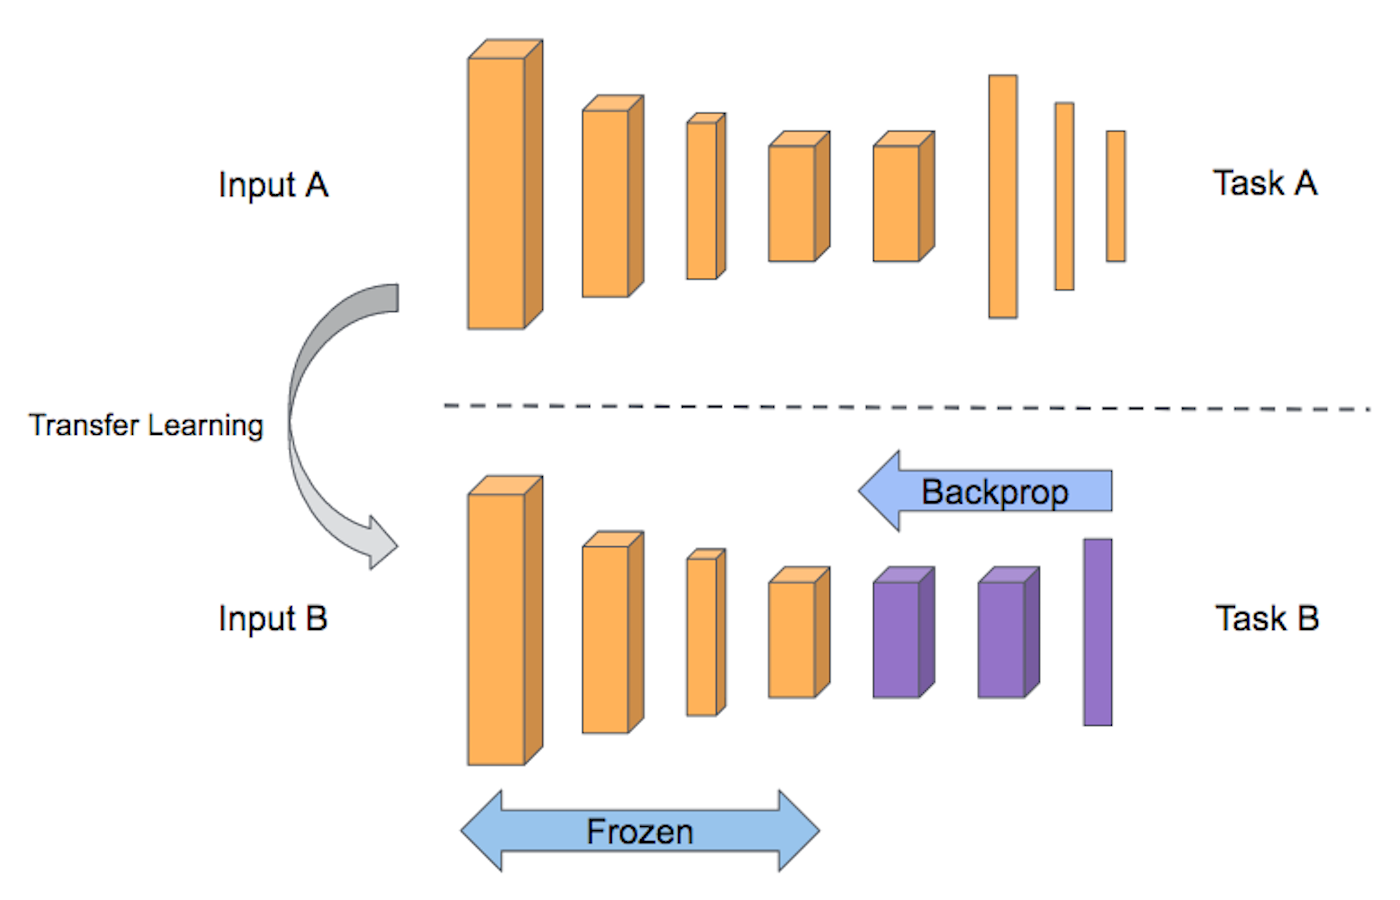
\includegraphics[width=9cm]{imgs/transfer_learning.png}
\end{figure}

\vspace{2mm}
\tiny{Fonte: \href{https://medium.com/@subodh.malgonde/transfer-learning-using-tensorflow-52a4f6bcde3e}{Transfer learning using Tensorflow} }

\end{frame}


%%%%%%%%%%%%%%%%%%%%%%%%%%%%%%%%%%%%%%%%%%%%%%%%%%%%%%%%%%%%%%%%%%%%%%%%%%%%%%%%%%%%%%%%%%%%%%%%%%%%%%%%%%%%%%%%
\section{Transfer Learning}
%%%%%%%%%%%%%%%%%%%%%%%%%%%%%%%%%%%%%%%%%%%%%%%%%%%%%%%%%%%%%%%%%%%%%%%%%%%%%%%%%%%%%%%%%%%%%%%%%%%%%%%%%%%%%%%%

\begin{frame}{Transfer Learning}

\begin{figure}[h]
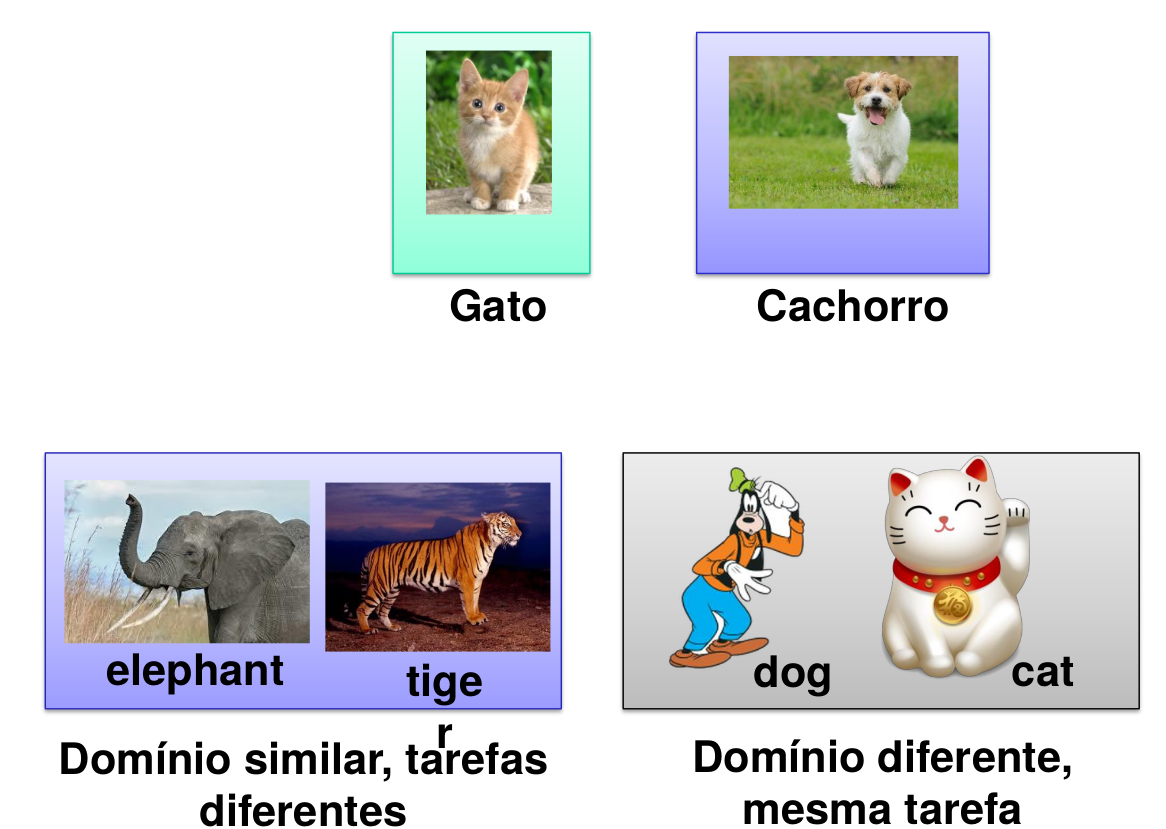
\includegraphics[width=8cm]{imgs/transfer_learning_domain.png}
\end{figure}

\end{frame}

%%%%%%%%%%%%%%%%%%%%%%%%%%%%%%%%%%%%%%%%%%%%%%%%%%%%%%%%%%%%%%%%%%%%%%%%%%%%%%%%%%%%%%%%%%%%%%%%%%%%%%%%%%%%%%%%

\begin{frame}{Transfer Learning}{Tarefas}

\begin{figure}[h]
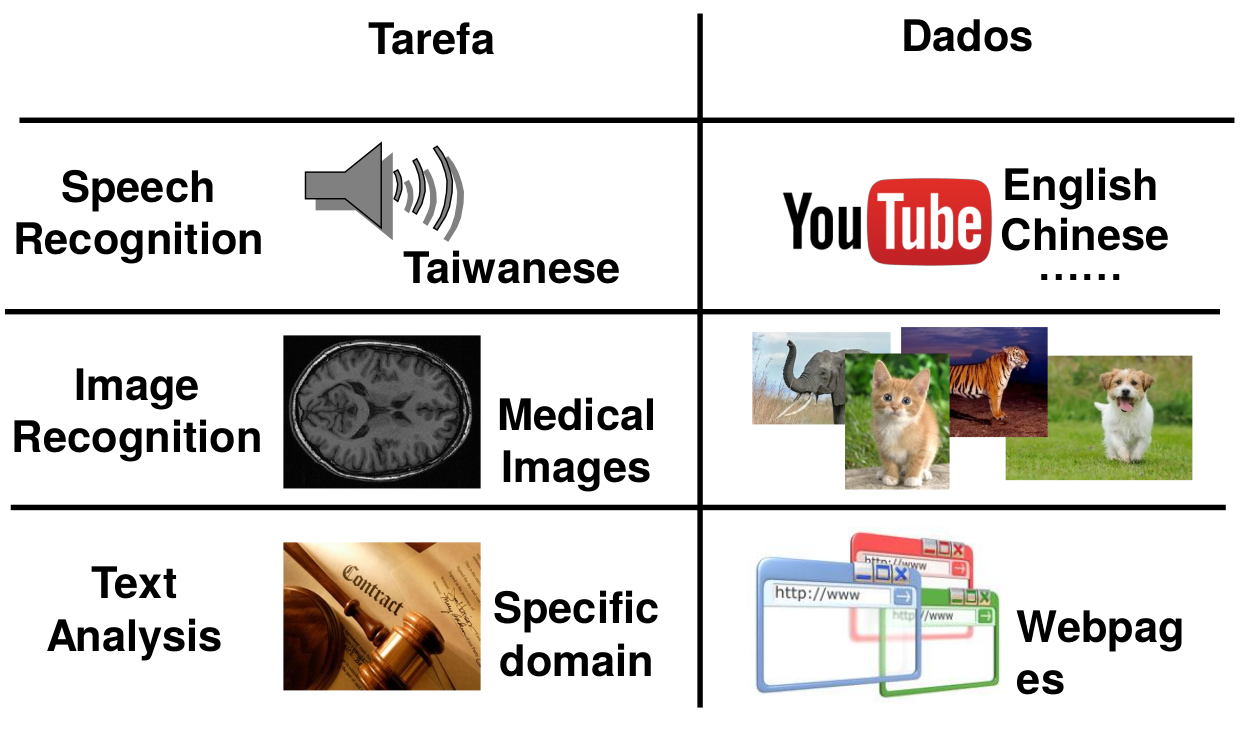
\includegraphics[width=8cm]{imgs/transfer_learning_tarefas.png}
\end{figure}

\end{frame}


%%%%%%%%%%%%%%%%%%%%%%%%%%%%%%%%%%%%%%%%%%%%%%%%%%%%%%%%%%%%%%%%%%%%%%%%%%%%%%%%%%%%%%%%%%%%%%%%%%%%%%%%%%%%%%%%

\begin{frame}{Transfer Learning}{Fine-Tuning}
\begin{itemize}
\item Tarefa
\begin{itemize}
\item Source data $(x^s, y^s)$: muitos dados.
\item Target data $(x^t, y^t)$: poucos dados.
\end{itemize}
\item Exemplo: classifica��o melanoma.
\begin{itemize}
\item Source data: ImageNet.
\item Target data: dataset espec�fico para melanoma.
\end{itemize}
\item Solu��o:
\begin{itemize}
\item Treinar o modelo em uma fonte grande de dados.
\item Fazer um ajuste fino ({\it fine tuning}) no modelo.
\item Cuidado com {\it overfitting}.
\end{itemize}
\end{itemize}
\end{frame}

%%%%%%%%%%%%%%%%%%%%%%%%%%%%%%%%%%%%%%%%%%%%%%%%%%%%%%%%%%%%%%%%%%%%%%%%%%%%%%%%%%%%%%%%%%%%%%%%%%%%%%%%%%%%%%%%

\begin{frame}{Transfer Learning}{Conservative Training}

\begin{figure}[h]
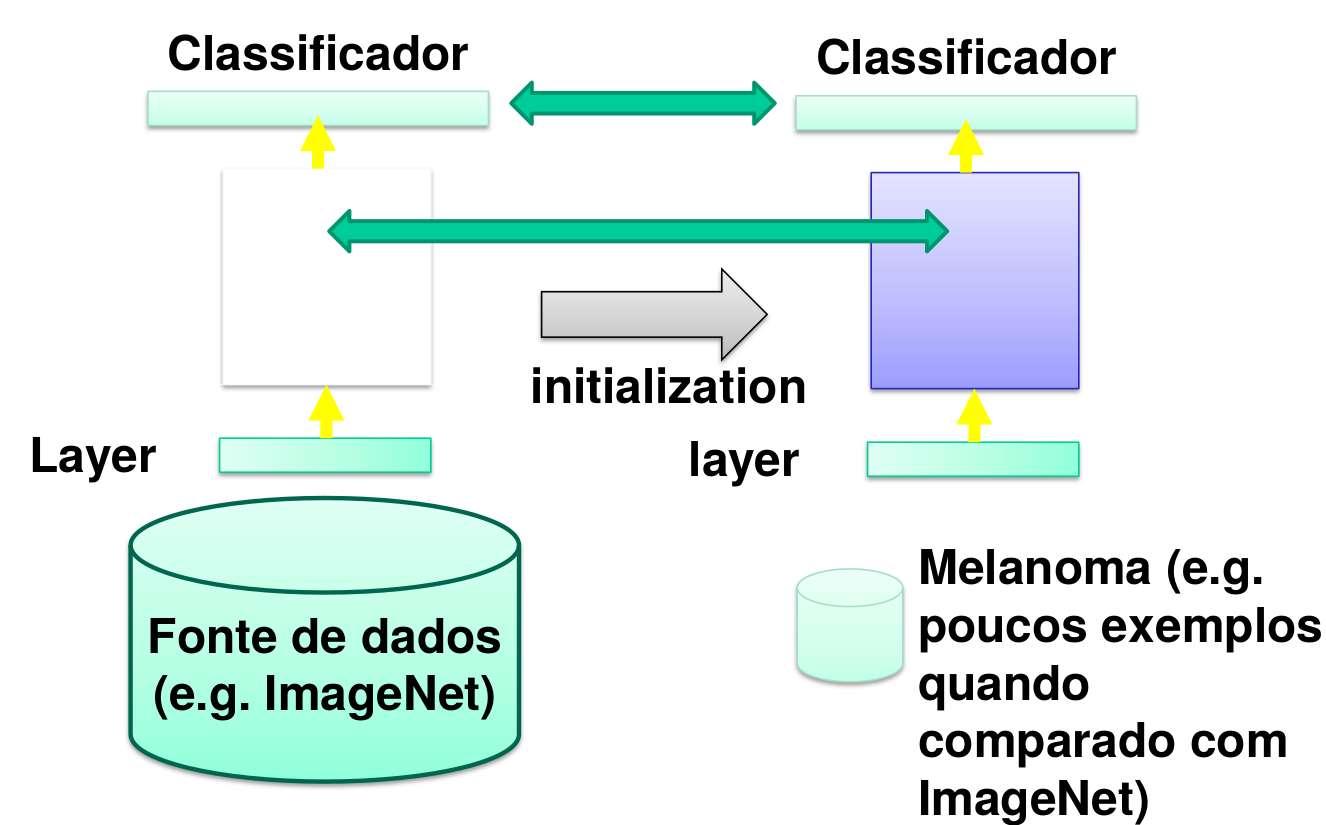
\includegraphics[width=8cm]{imgs/transfer_learning_convervative_training.png}
\end{figure}

\end{frame}

%%%%%%%%%%%%%%%%%%%%%%%%%%%%%%%%%%%%%%%%%%%%%%%%%%%%%%%%%%%%%%%%%%%%%%%%%%%%%%%%%%%%%%%%%%%%%%%%%%%%%%%%%%%%%%%%

\begin{frame}{Transfer Learning}{Layer Transfer}
Quais camadas devem ser transferidas?
\begin{itemize}
\item Imagem: geralmente as primeiras camadas.
\item Texto: geralmente as �ltimas camadas.
\end{itemize}
\begin{figure}[h]
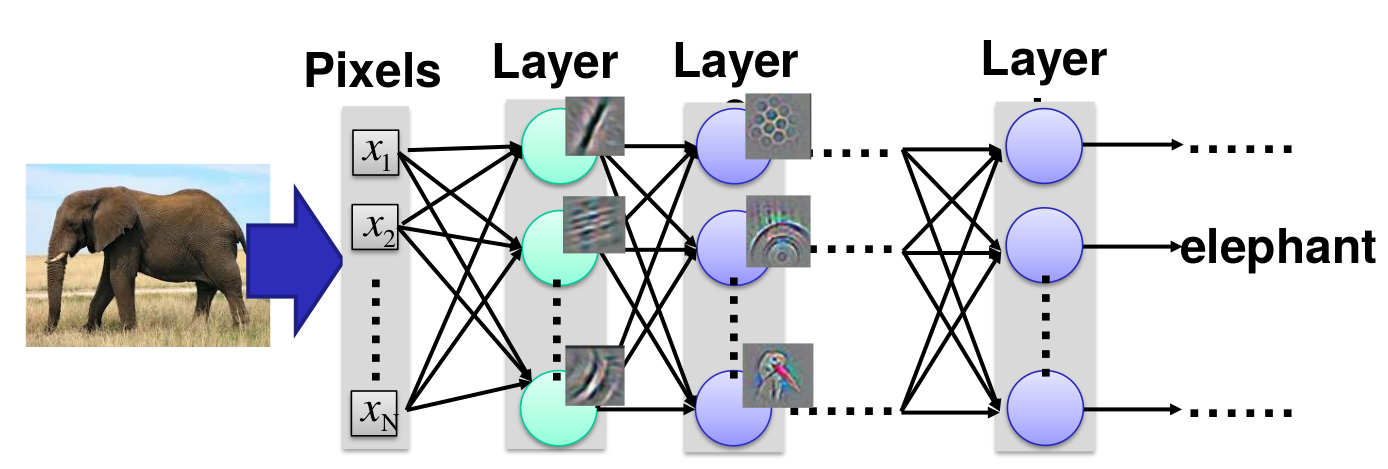
\includegraphics[width=8cm]{imgs/transfer_learning_layer_transfer.png}
\end{figure}

\end{frame}

%%%%%%%%%%%%%%%%%%%%%%%%%%%%%%%%%%%%%%%%%%%%%%%%%%%%%%%%%%%%%%%%%%%%%%%%%%%%%%%%%%%%%%%%%%%%%%%%%%%%%%%%%%%%%%%%

\begin{frame}{Transfer Learning}{Strategy}

\begin{figure}[h]
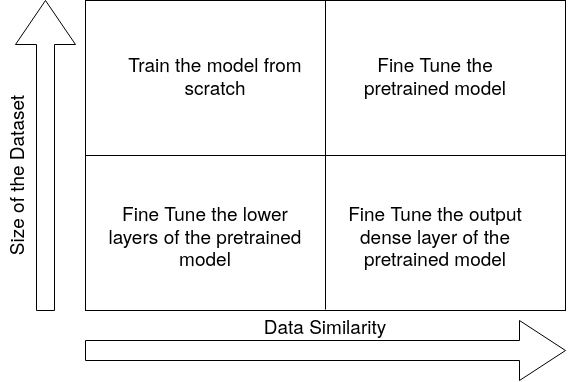
\includegraphics[width=6cm]{imgs/transfer_learning_strategy.png}
\end{figure}

\end{frame}

%%%%%%%%%%%%%%%%%%%%%%%%%%%%%%%%%%%%%%%%%%%%%%%%%%%%%%%%%%%%%%%%%%%%%%%%%%%%%%%%%%%%%%%%%%%%%%%%%%%%%%%%%%%%%%%%

\begin{frame}{Transfer Learning}{Cen�rio 1}
{\bf Cen�rio 1}
\begin{itemize}
\item Data set pequeno e a similaridade dos dados � muito alta.
\begin{itemize}
\item Use a rede pretreinada como {\it feature extractor}.
\end{itemize}
\item Exemplo: Suponha que vamos usar uma rede treinada para um novo conjunto de gatos e cachorros.
\begin{itemize}
\item ImageNet: 1000 classes de sa�da.
\item Modificamos a �ltimas camadas ({\it dense layers}) e a fun��o de ativa��o ({\it softmax}) para duas categorias ({\it sigmoid}).
\end{itemize}
\end{itemize}
\end{frame}

%%%%%%%%%%%%%%%%%%%%%%%%%%%%%%%%%%%%%%%%%%%%%%%%%%%%%%%%%%%%%%%%%%%%%%%%%%%%%%%%%%%%%%%%%%%%%%%%%%%%%%%%%%%%%%%%

\begin{frame}{Transfer Learning}{Cen�rio 2}
{\bf Cen�rio 2}
\begin{itemize}
\item Data set pequeno e similaridade de dados baixa.
\item Mantenha as camadas iniciais da rede pretreinada.
\item Retreine as camadas intermedi�rias e finais.
\end{itemize}
\end{frame}


%%%%%%%%%%%%%%%%%%%%%%%%%%%%%%%%%%%%%%%%%%%%%%%%%%%%%%%%%%%%%%%%%%%%%%%%%%%%%%%%%%%%%%%%%%%%%%%%%%%%%%%%%%%%%%%%

\begin{frame}{Transfer Learning}{Cen�rio 3}
{\bf Cen�rio 3}
\begin{itemize}
\item Data set grande e similaridade de dados baixa.
\item Neste caso.... Fuja para as montanhas...
\end{itemize}

\begin{figure}[h]
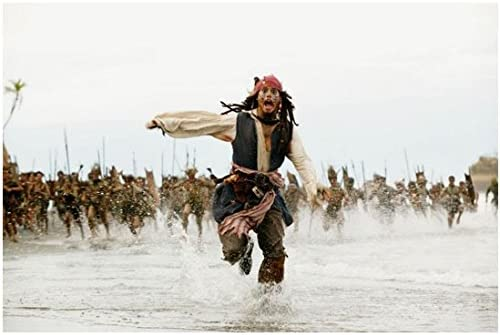
\includegraphics[width=6cm]{imgs/run_to_the_hills.jpg}
\end{figure}

\end{frame}

%%%%%%%%%%%%%%%%%%%%%%%%%%%%%%%%%%%%%%%%%%%%%%%%%%%%%%%%%%%%%%%%%%%%%%%%%%%%%%%%%%%%%%%%%%%%%%%%%%%%%%%%%%%%%%%%

\begin{frame}{Transfer Learning}{Cen�rio 4}
{\bf Cen�rio 3}
\begin{itemize}
\item Data set grande e alta similaridade.
\item Situa��o ideal: no m�ximo treinar o classificador no topo da rede.
\end{itemize}

\begin{figure}[h]

\includegraphics[width=4cm]{imgs/easy_win.jpg}
\end{figure}

\end{frame}


%%%%%%%%%%%%%%%%%%%%%%%%%%%%%%%%%%%%%%%%%%%%%%%%%%%%%%%%%%%%%%%%%%%%%%%%%%%%%%%%%%%%%%%%%%%%%%%%%%%%%%%%%%%%%%%%

\begin{frame}{Refer�ncias}
\begin{itemize}
\item A Newbie-Friendly Guide to Transfer Learning
\begin{itemize}
\item \url{https://www.v7labs.com/blog/transfer-learning-guide}
\end{itemize}
\item A Comparison of 4 Popular Transfer Learning Models
\begin{itemize}
\item \url{https://analyticsindiamag.com/a-comparison-of-4-popular-transfer-learning-models/}
\end{itemize}
\end{itemize}
\end{frame}


%%%%%%%%%%%%%%%%%%%%%%%%%%%%%%%%%%%%%%%%%%%%%%%%%%%%%%%%%%%%%%%%%%%%%%%%%%%%%%%%%%%%%%%%%%%%%%%%%%%%%%%%%%%%%%%%

\begin{frame}[plain]
  \titlepage
\end{frame}



\end{document}
